
\subsection{Noise Robustness Comparisons}

Here we present results for noise robustness experiments. Tests were performed by transforming data by various transforms, and adding different amounts of noise. Noise here is measured in both SNR and noise range. A noise range of 1.0 means random noise within the range [$-0.5$, $0.5$] was added. SNR is measured in decibels. 

\begin{figure*}[t]
\centering
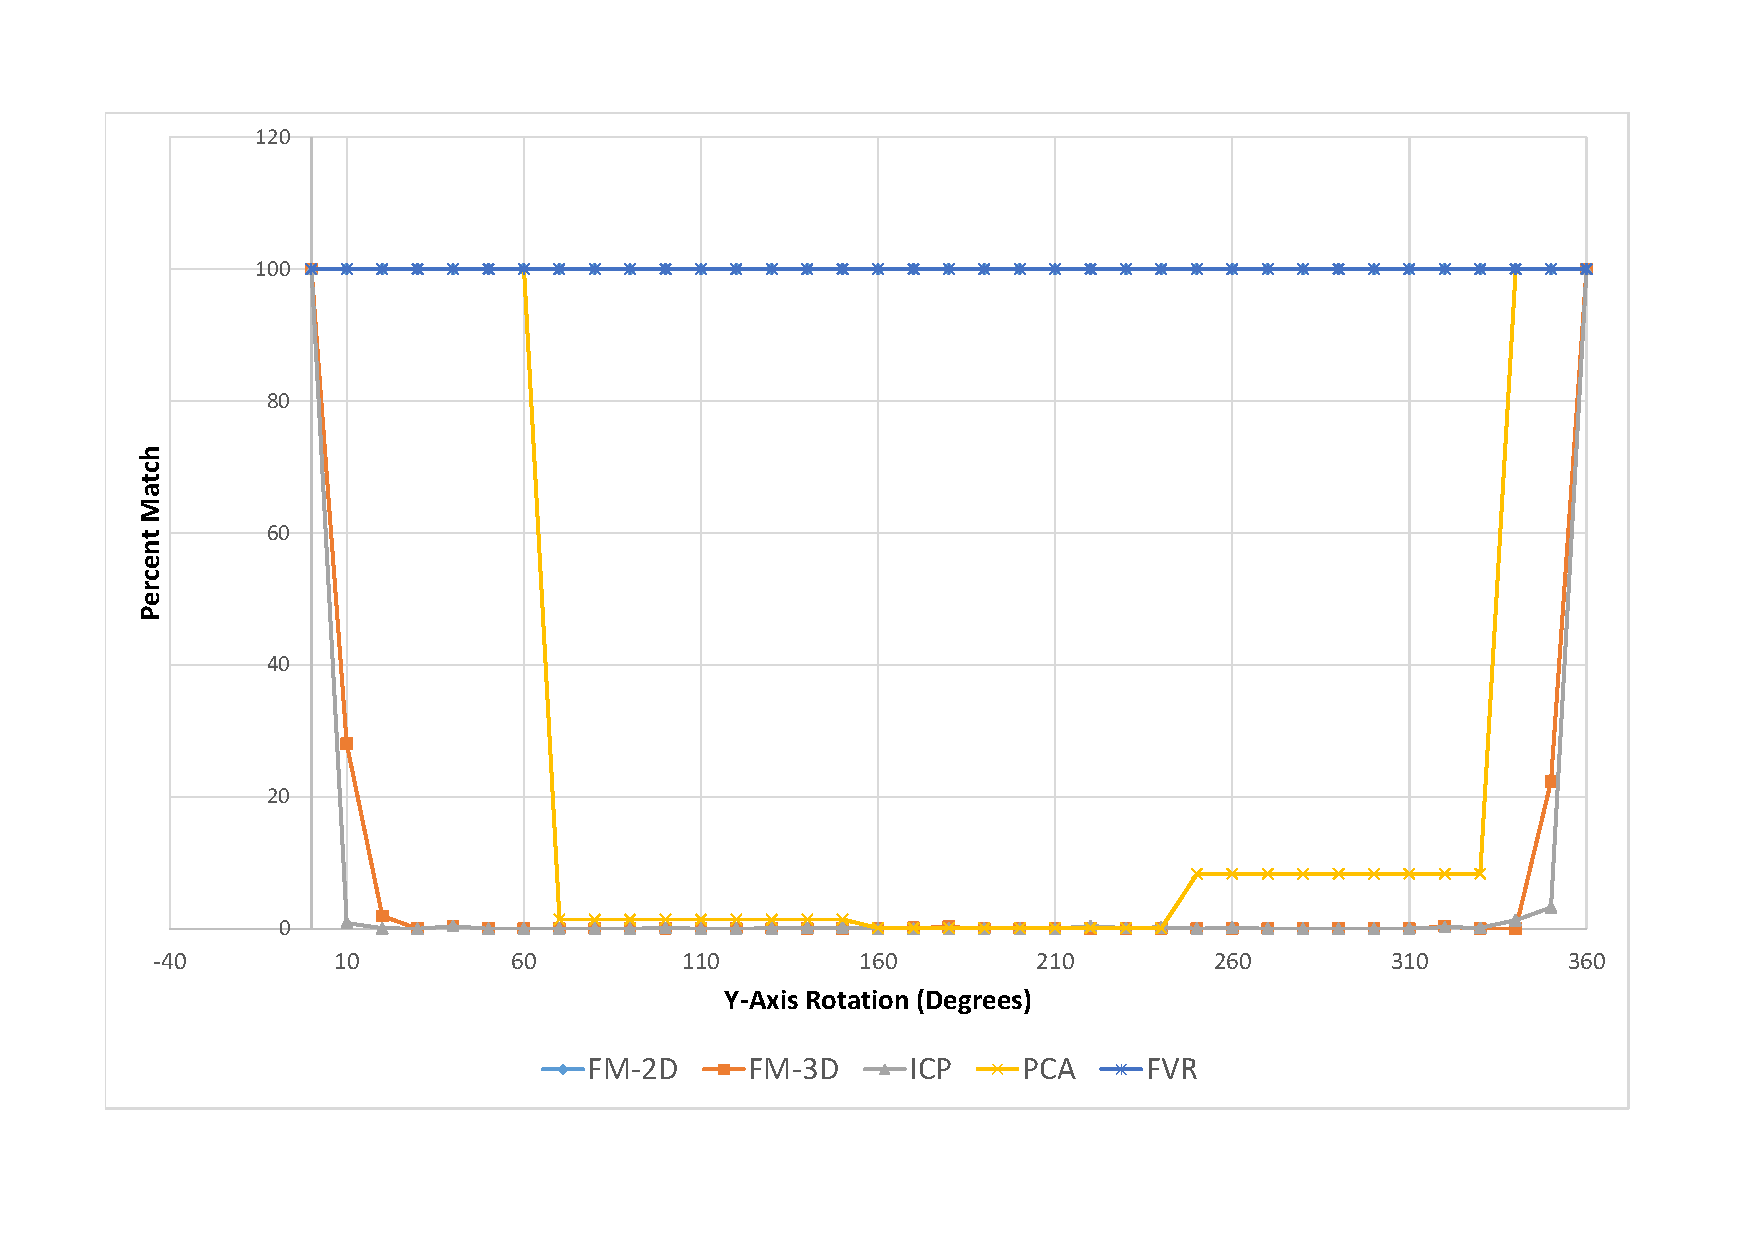
\includegraphics[width=6.0in]{images/results/noise/YRNoise0}
\caption{Percent Match for Y-Axis Registration with an Infinite SNR and noise range of $0$.}
\label{fig:YRNoise0}
\end{figure*}

In the first set of experiments, scanned 3D data was rotated about the Y-axis. Figure \ref{fig:YRNoise0} shows results with an infinite SNR. The 2D-FM method and FVR achieved perfect results. PCA performed next best, but failed to register degrees above 70. Since no noise was present, PCA was truly accurate, however some axes were flipped. This may be fixed by testing the data for flipped axes. FM-3D and ICP fell away much earlier. ICP is not good at registering significant transforms and FM-3D also does not perform well as quantization errors are higher since we use volume sizes of $128^3$.

\begin{figure*}[t]
\centering
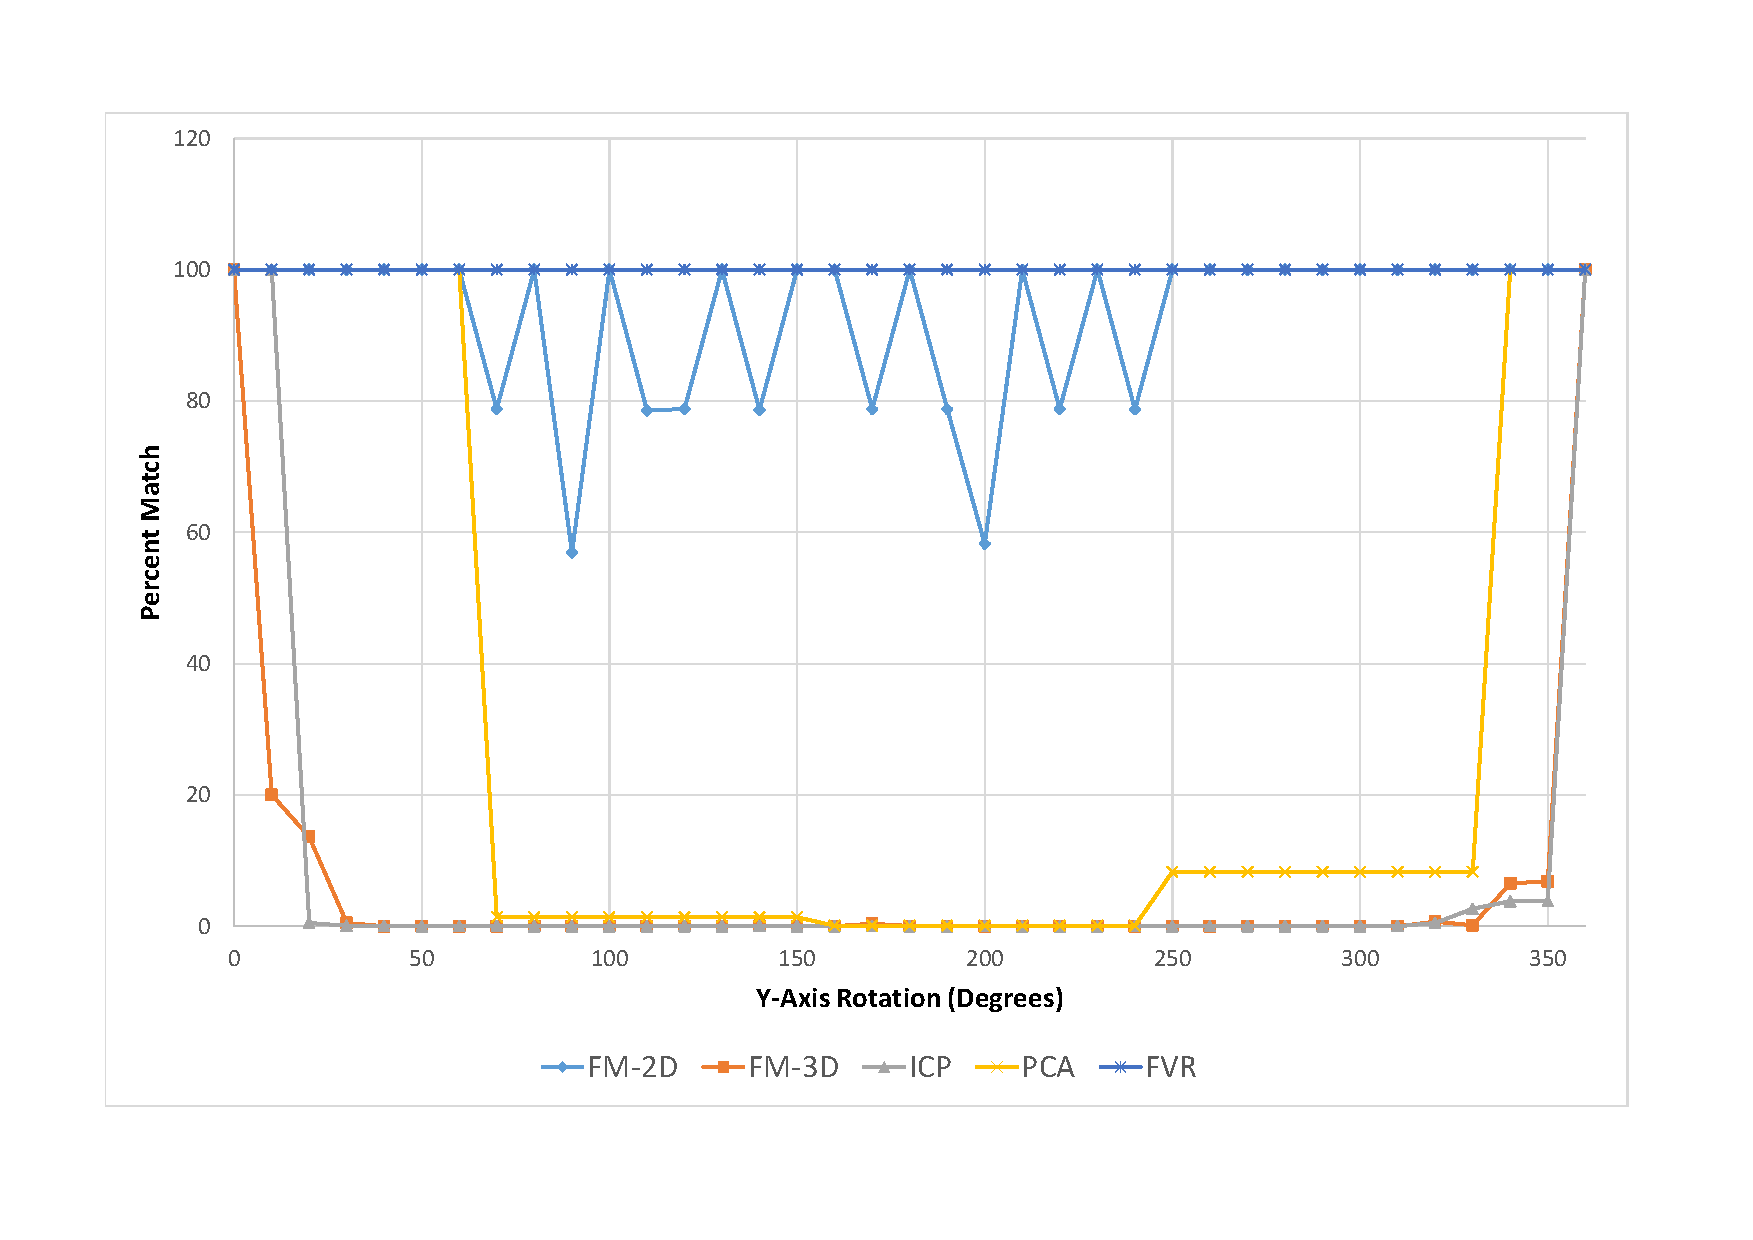
\includegraphics[width=6.0in]{images/results/noise/YRNoise1}
\caption{Percent Match for Y-Axis Registration with an SNR of and noise range of $10300$ and noise range of $1.0$.}
\label{fig:YRNoise1}
\end{figure*}

For the results in figure \ref{fig:YRNoise1} we dropped the SNR to $10300$. Here we see similar results but FM-2D has begun to show some errors with larger rotations (remember rotations above 180 can be considered smaller but negative rotations). In figure \ref{fig:YRNoise2} we reduced the SNR to $2580$ which caused more error in FM-2D. These results suggest that for simple Y-axis rotation, FVR is superior in terms of noise robustness. 

\begin{figure*}[t]
\centering
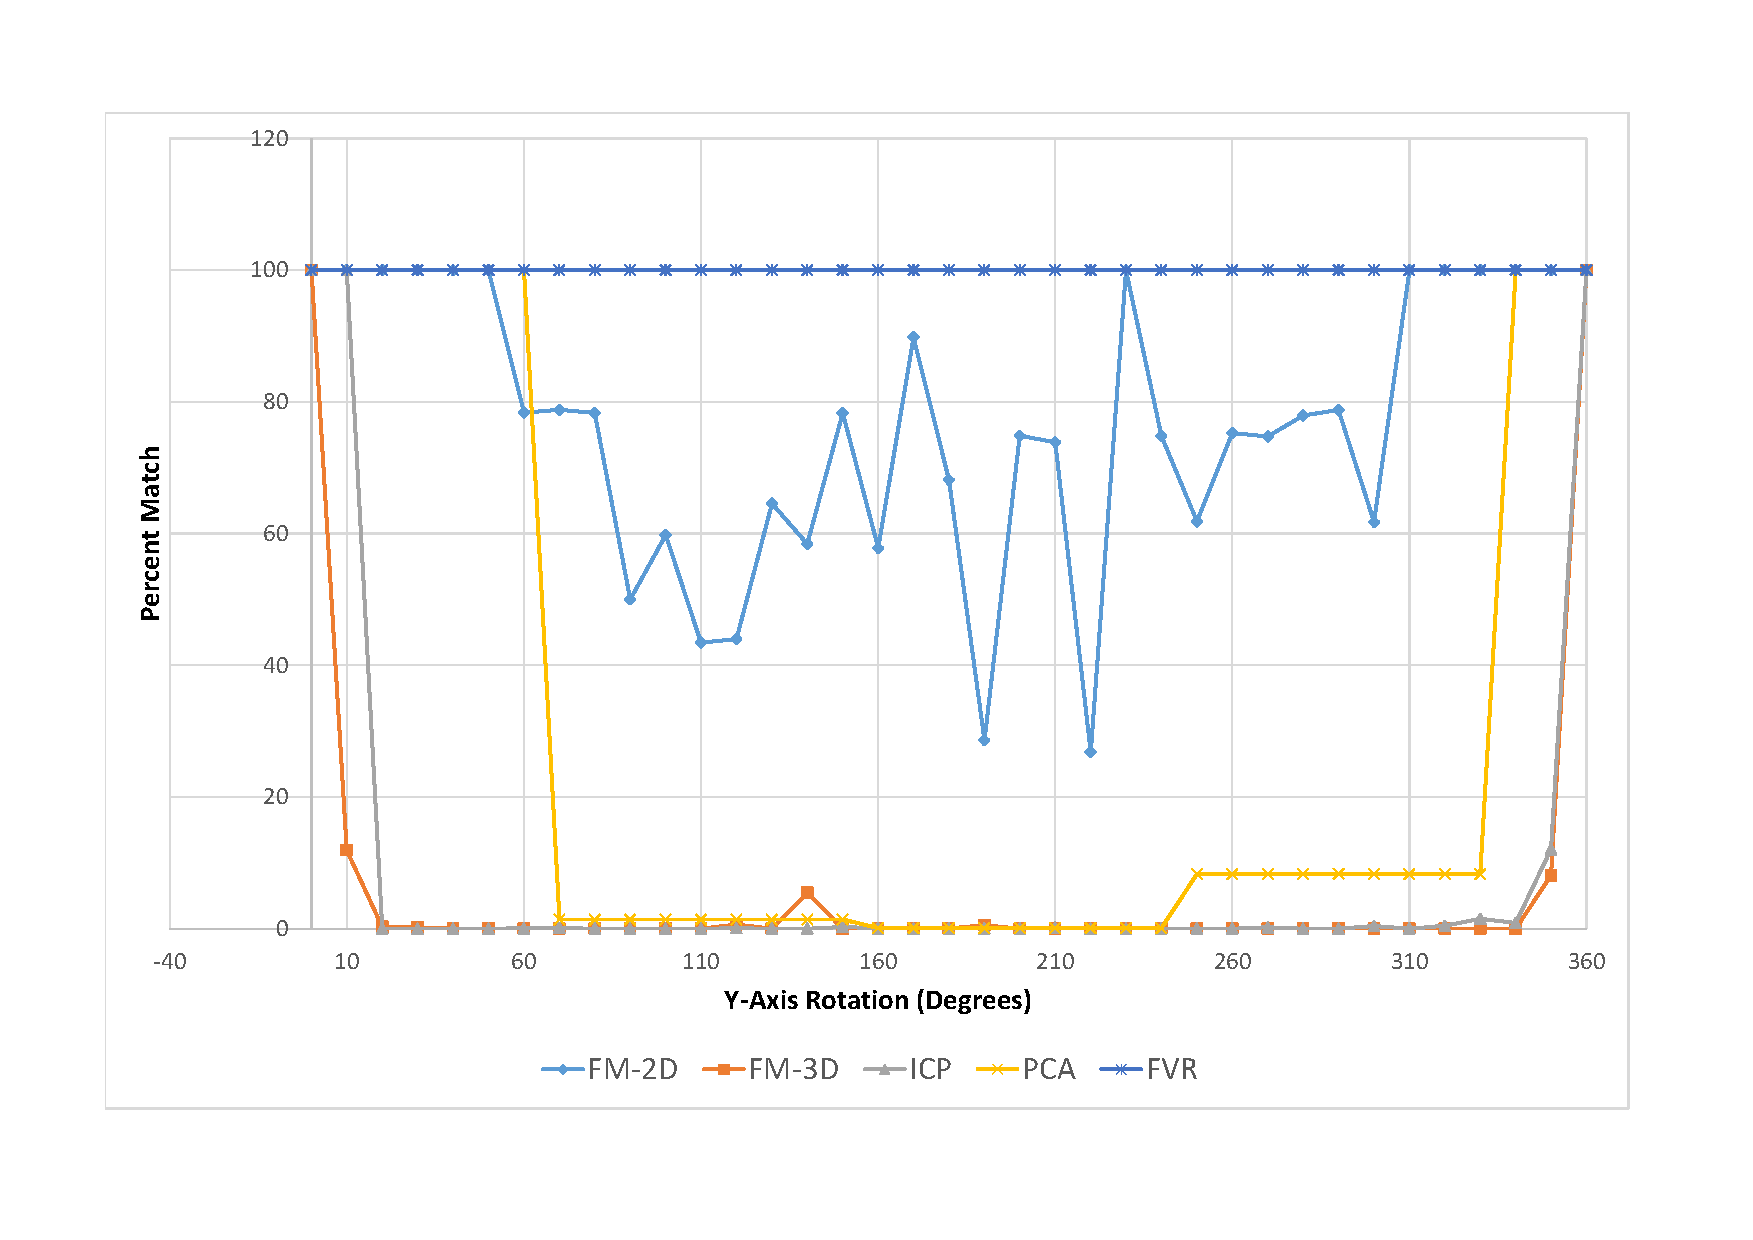
\includegraphics[width=6.0in]{images/results/noise/YRNoise2}
\caption{Percent Match for Y-Axis Registration with an SNR of 2580 and noise range of $2.0$.}
\label{fig:YRNoise2}
\end{figure*}


\begin{figure*}[t]
\centering
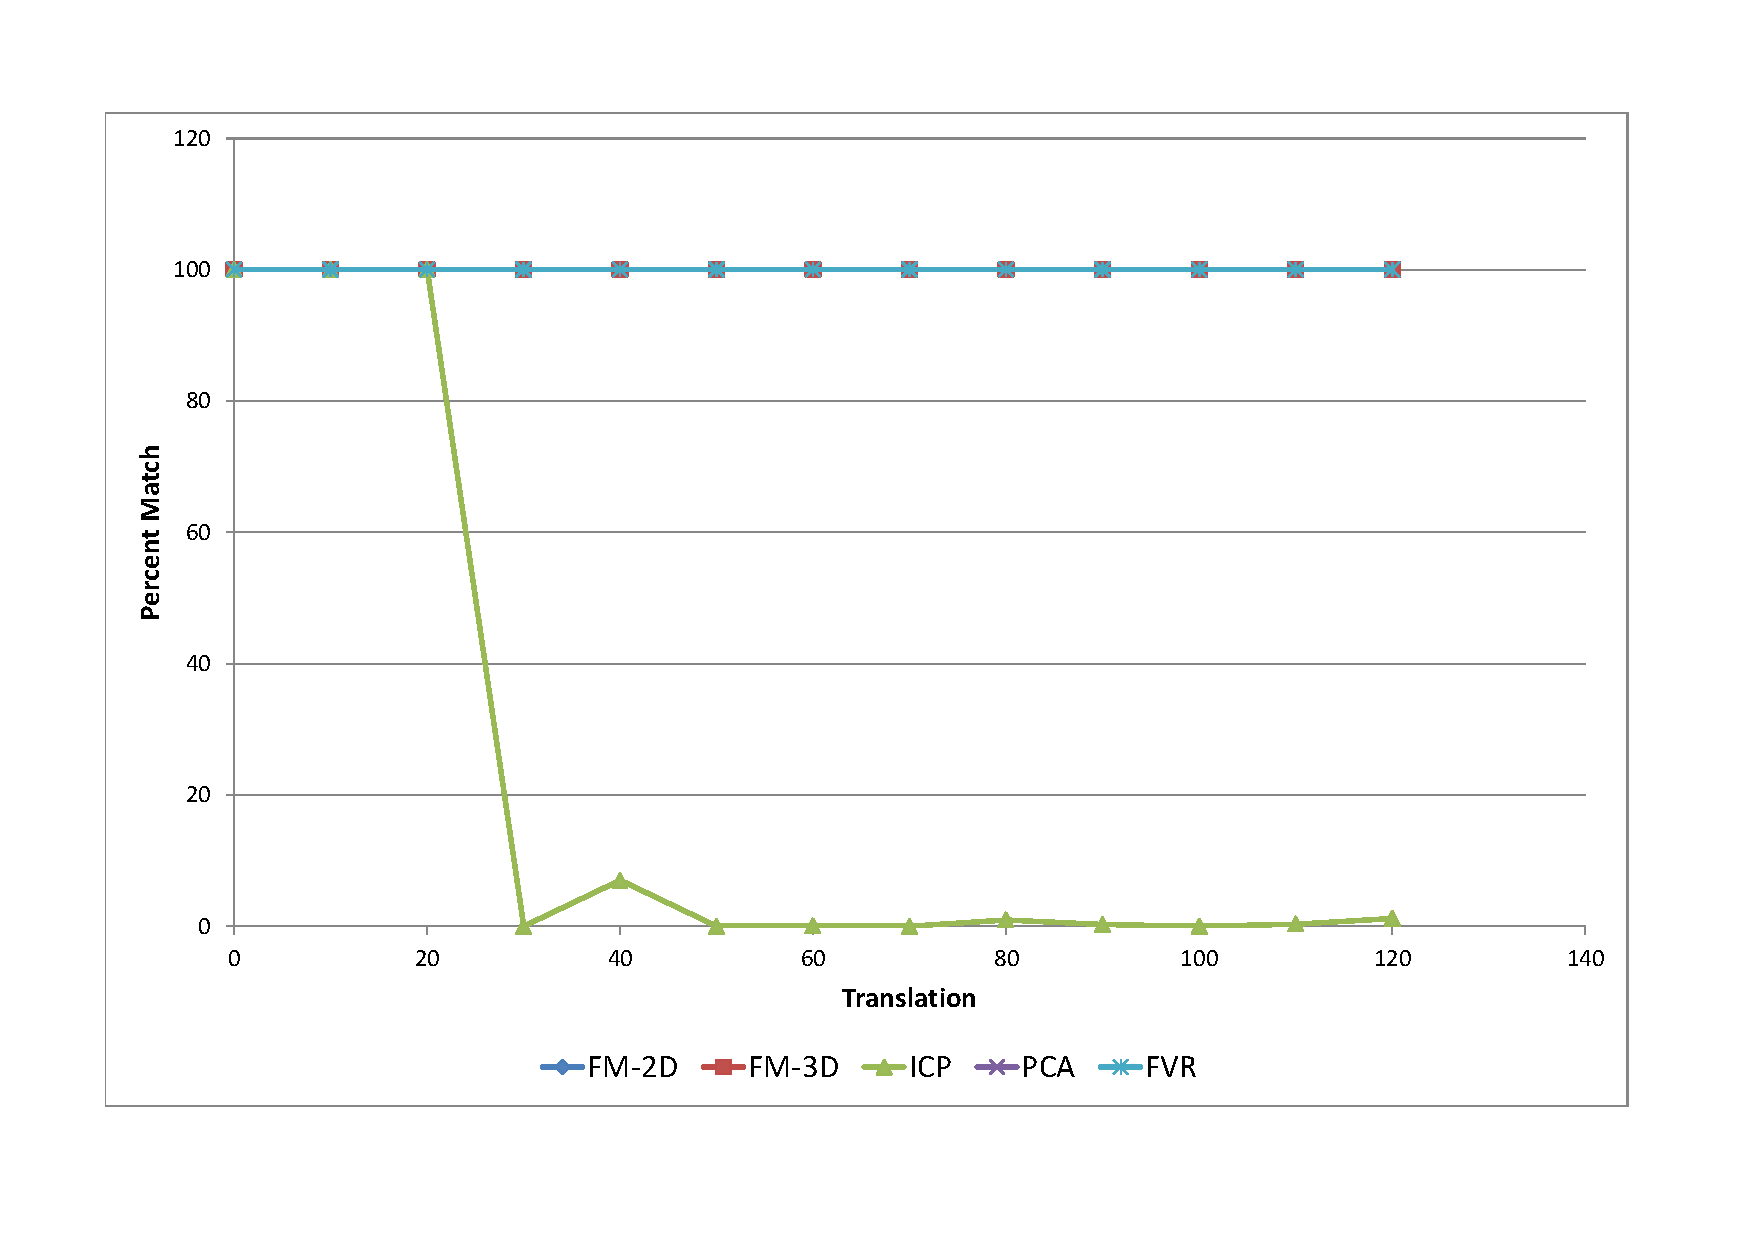
\includegraphics[width=6.0in]{images/results/noise/TransNoise0}
\caption{Percent Match for Translation Registration with an infinite SNR and noise range of $0$.}
\label{fig:TNoise0}
\end{figure*}


\begin{figure*}[t]
\centering
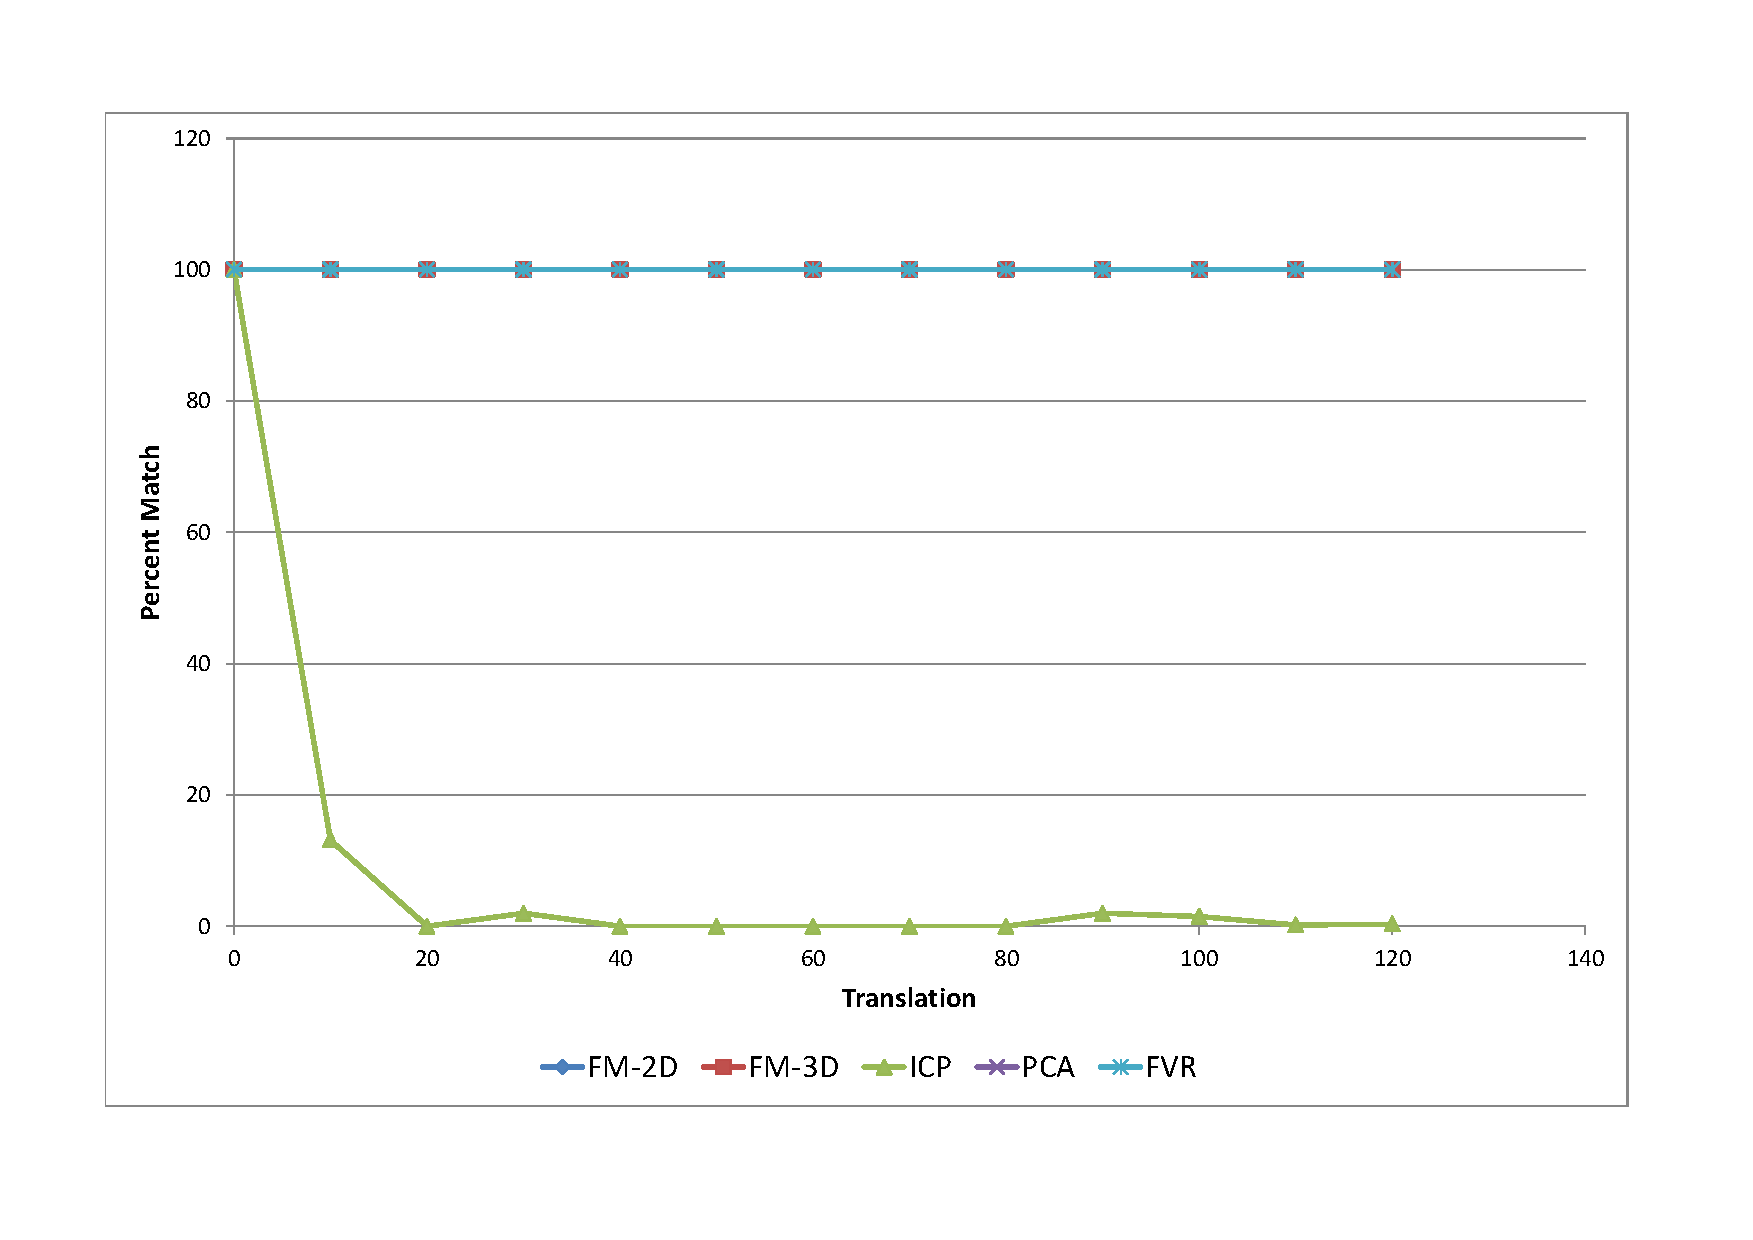
\includegraphics[width=6.0in]{images/results/noise/TransNoise1}
\caption{Percent Match for Translation Registration with an SNR of and noise range of $10300$ and noise range of $1.0$.}
\label{fig:TNoise1}
\end{figure*}


\begin{figure*}[t]
\centering
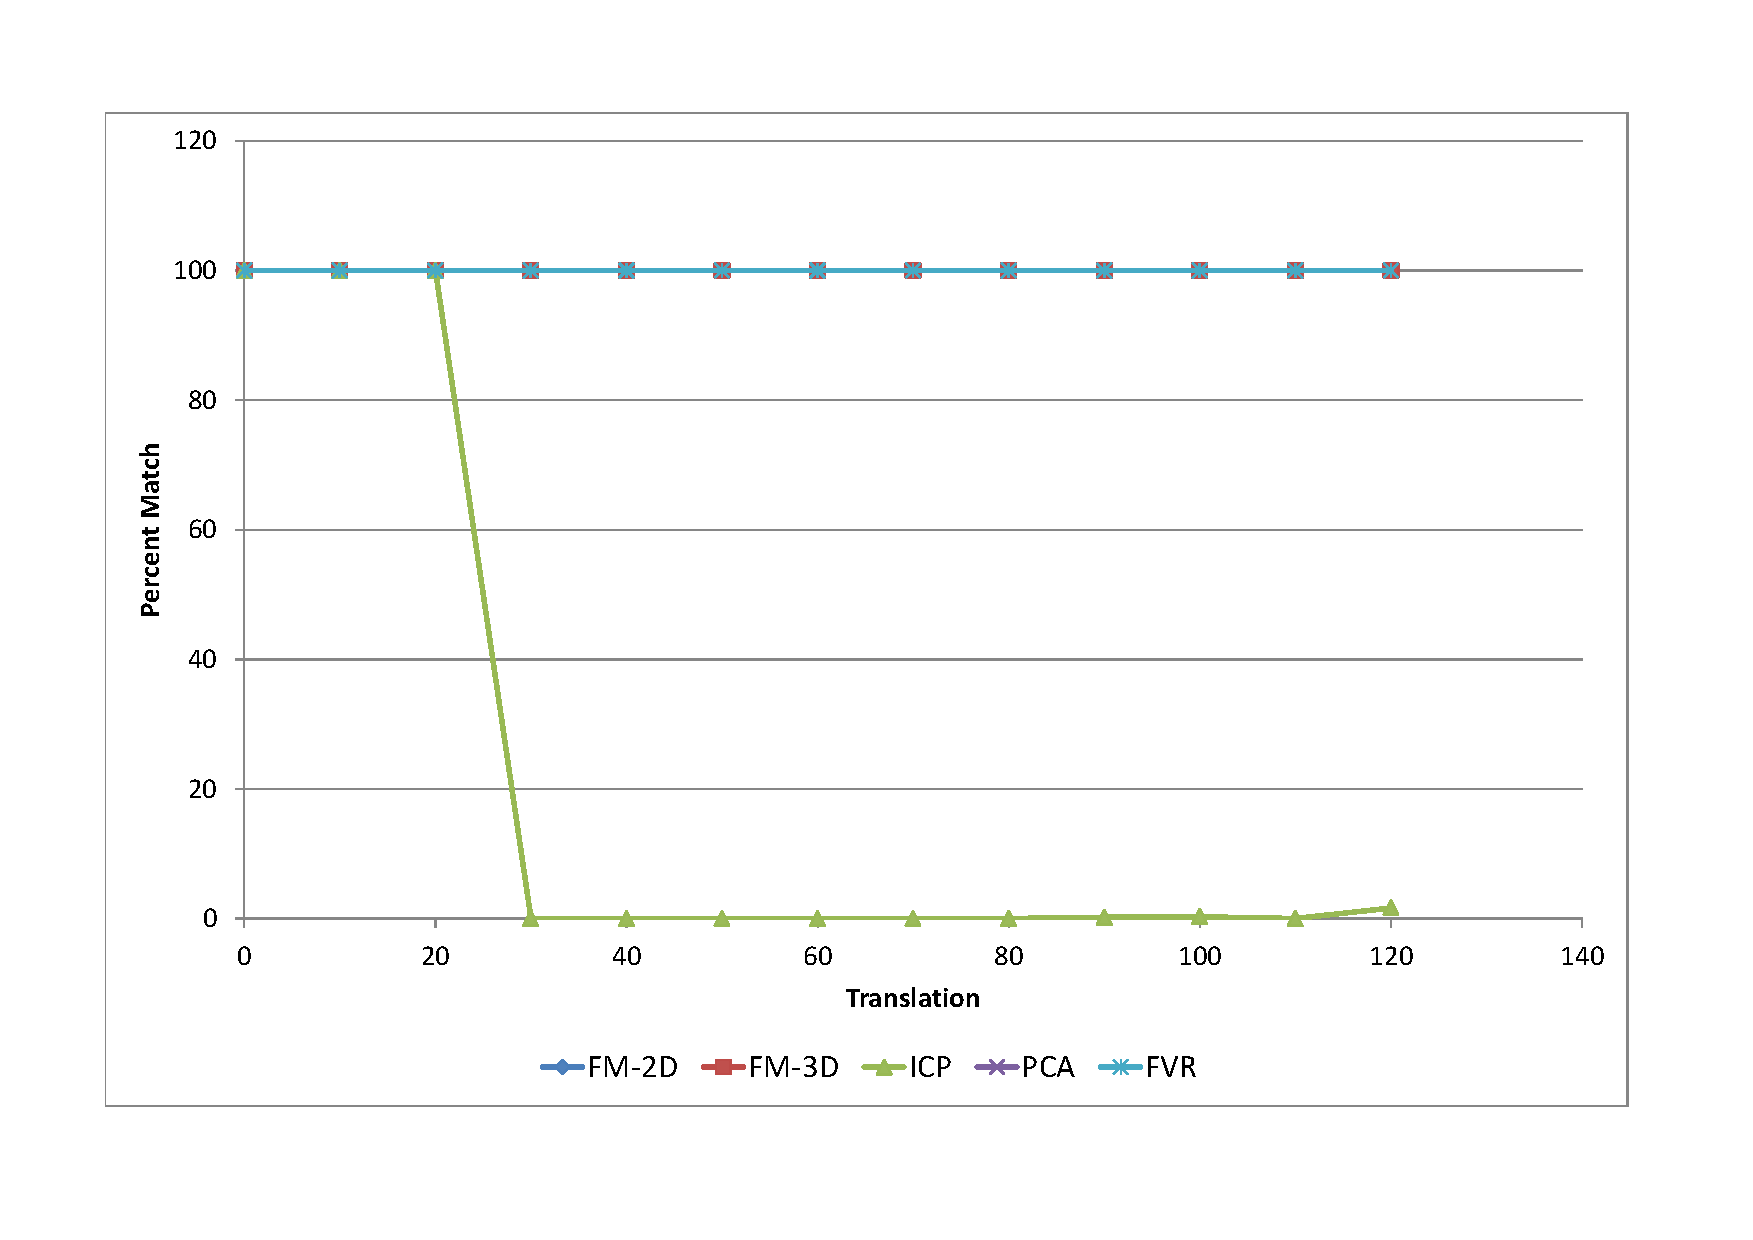
\includegraphics[width=6.0in]{images/results/noise/TransNoise2}
\caption{Percent Match for Translation Registration with an SNR of and noise range of $2580$ and noise range of $2.0$.}
\label{fig:TNoise2}
\end{figure*}